\section{Splines in Bernstein-Bézier Form}

\begin{exercise}
    Prove equation~(2.8).
\end{exercise}

\begin{solution}
    Equation~(2.8) states that the condition for $C^2$ continuity of $s$ can be expressed as the two equations in (2.7), namely
    \begin{equation*}
        e_0 = c_d \quad \text{and} \quad e_1 = (1 - \alpha) c_d + \alpha c_{d-1}
    \end{equation*}
    where
    \begin{equation*}
        \alpha = \frac{c - a}{b - a},
    \end{equation*}
    plus the equation
    \begin{equation*}
        e_2 = (1 - \alpha)^2 c_d + 2(1 - \alpha) \alpha c_{d-1} + \alpha^2 c_{d-2}.
    \end{equation*}

    In the original theorem, we have that a spline $s$ has $C^r$ continuity, for $r = 0, 1, \ldots, d$, if and only if
    \begin{equation*}
        \frac{1}{(b - a)^k} \Delta^k c_{d - k} = \frac{1}{(c - b)^k} \Delta^k e_0, \qquad k = 0, 1, \ldots, r.
    \end{equation*}

    For $r = 2$, we must then solve for $k = 0, 1, 2$.
    In the first case we simply have
    \begin{align*}
        \frac{1}{(b - a)^0} \Delta^0 c_d &= \frac{1}{(c - b)^0} \Delta^0 e_0, \\
        c_d &= e_0.
    \end{align*}
    For $k = 1$ we have then have
    \begin{align*}
        \frac{1}{(b - a)^1} \Delta^1 c_{d - 1} &= \frac{1}{(c - b)^1} \Delta^1 e_0, \\
        \frac{c_d - c_{d-1}}{b - a} &= \frac{e_1 - e_0}{c - b} = \frac{e_1 - c_d}{c - b}, \\
        e_1 - c_d &= \frac{c - b}{b - a} (c_{d-1} - c_d), \\
        e_1 &= (1 - \alpha) c_d + \alpha c_{d-1}.
    \end{align*}
    Finally, for $k = 2$ we have
    \begin{align*}
        \frac{1}{(c - b)^2} \Delta^2 e_0, &= \frac{1}{(b - a)^2} \Delta^2 c_{d - 2} \\
        \frac{e_2 - 2 e_1 + e_0}{(c-b)^2} &= \frac{c_{d} - 2 c_{d-1} + c_{d-2}}{(b-a)^2}, \\
        e_2 - 2 \left( (1 - \alpha) c_d + \alpha c_{d-1} \right) + c_d &= \alpha^2 \left( c_{d-2} - 2 c_{d-1} + c_d \right) \\
        e_2 &= \left( \alpha^2 - 2 \alpha + 1 \right) c_d + 2 \left( \alpha - \alpha^2 \right) c_{d-1} + \alpha^2 c_{d-2} \\
        e_2 &= (1 - \alpha)^2 c_d + 2(1 - \alpha) \alpha c_{d-1} + \alpha^2 c_{d-2},
    \end{align*}
    which is the desired result.
\end{solution}

\begin{exercise}\label{ex:bezier_spline}
    Implement the de Casteljau algorithm for a planar Bézier curve of arbitrary degree $d$ over a general interval $[a, b]$.
    Use the routine to make a program to plot the quadratic spline curve $\mathbf{s} : [0, 2] \to \mathbb{R}$, with pieces
    \begin{align*}
        \mathbf{p}(t) &= \sum_{i=0}^{2} \mathbf{c}_i B_{i}^2(t), & 0 \leq t \leq 1, \\
        \mathbf{q}(t) &= \sum_{i=0}^{2} \mathbf{d}_i B_{i}^2(t - 1), & 1 < t \leq 2,
    \end{align*}
    where $\mathbf{c}_0 = (-1, 1)$, $\mathbf{c}_1 = (-1, 0)$, $\mathbf{c}_2 = (0, 0)$, and $\mathbf{d}_0 = (0, 0)$, $\mathbf{d}_1 = (1, 0)$, $\mathbf{d}_2 = (2, 1)$.
\end{exercise}

\begin{solution}
    The de Casteljau algorithm is implemented in \verb|spline_cj.py|, and is practically identical to the one implemented in the previous section, due to the vectorization possibilities in \verb|JAX|.
    The resulting figure is shown in Figure~\ref{fig:bezier_spline}.
    \begin{figure}[ht]
        \centering
        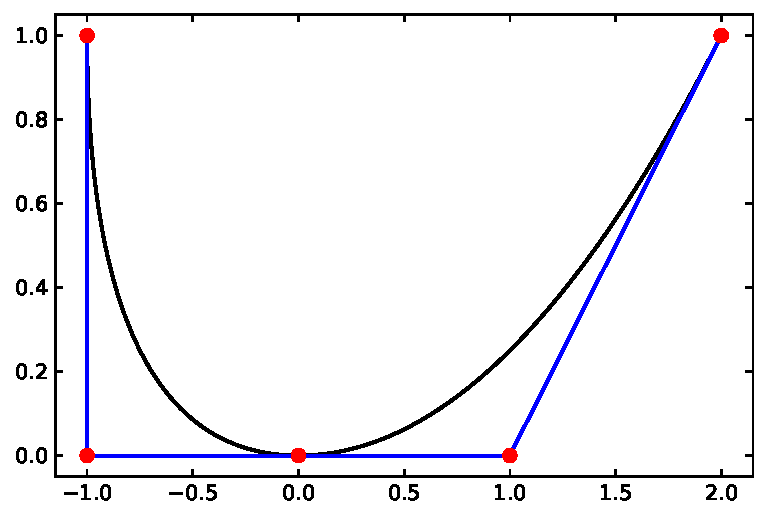
\includegraphics[width=0.7\textwidth]{2_splines_in_bb/bezier_casteljau.pdf}
        \caption{The quadratic spline curve $\mathbf{s} : [0, 2] \to \mathbb{R}$, with pieces $\mathbf{p}(t)$ and $\mathbf{q}(t)$.\label{fig:bezier_spline}}
    \end{figure}
\end{solution}

\begin{exercise}
    What is the order of continuity of $\mathbf{s}$ in Exercise~\ref{ex:bezier_spline} at the breakpoint $t = 1$?
\end{exercise}

\begin{solution}
    We clearly have $C^0$ continuity at the breakpoint $t = 1$, as
    \begin{equation*}
        \mathbf{c}_2 = (0, 0) = \mathbf{d}_0.
    \end{equation*}
    For $C^1$ continuity, we must have
    \begin{align*}
        \frac{\mathbf{c}_2 - \mathbf{c}_1}{1 - 0} &= \frac{\mathbf{d}_1 - \mathbf{d}_0}{2 - 1} \\
        (0, 0) - (-1, 0) &= (1, 0) - (0, 0),
    \end{align*}
    which also holds.
    Finally for $C^2$ continuity, we must have
    \begin{align*}
        \frac{\mathbf{c}_2 - 2 \mathbf{c}_1 + \mathbf{c}_0}{1^2} &\stackrel{?}{=} \frac{\mathbf{d}_2 - 2 \mathbf{d}_1 + \mathbf{d}_0}{1^2} \\
        (0, 0) - 2(-1, 0) + (-1, 1) = (1, 1) &\neq (0, 1) = (2, 1) - 2(1, 0) + (0, 0),
    \end{align*}
    which it seems like we do not have.
    Thus, the order of continuity of $\mathbf{s}$ at the breakpoint $t = 1$ is $C^1$.
\end{solution}

\begin{exercise}
    The curvature of a parametric curve $\mathbf{r}(t)$ in $\mathbb{R}^2$ can be expressed as
    \begin{equation*}
        \kappa(t) = \frac{\mathbf{r}'(t) \times \mathbf{r}''(t)}{\norm{\mathbf{r}'(t)}^3},
    \end{equation*}
    where $(a_1, a_2) \times (b_1, b_2) := a_1 b_2 - a_2 b_1$.
    What are the curvatures of $\mathbf{p}$ and $\mathbf{q}$ in Exercise~\ref{ex:bezier_spline} at the breakpoint $t = 1$?
    What can you say about the smoothness of $\mathbf{s}$?
\end{exercise}

\begin{solution}
    We firstly begin by tabulating the derivatives of $\mathbf{p}$ and $\mathbf{q}$, based on the general formula
    \begin{equation*}
        p^{(r)}(x) = \frac{d!}{(d - r)!} \frac{1}{h^r} \sum_{i=0}^{d-r} \Delta^r c_{i} B_i^{d-r}(\lambda).
    \end{equation*}
    In both cases here, we have $h = 1$, $d = 2$, and $\lambda = t$ for $\mathbf{p}$ and $\lambda = t - 1$ for $\mathbf{q}$.
    The derivatives for $\mathbf{p}$ are then
    \begin{align*}
        \mathbf{p}'(t) &= 2 \left(\left( \mathbf{c}_1 - \mathbf{c}_0 \right) B_0^1(\lambda) + \left( \mathbf{c}_2 - \mathbf{c}_1 \right) B_1^1(\lambda)\right) &
        \mathbf{p}''(t) &= 2 \left( \mathbf{c}_2 - 2 \mathbf{c}_1 + \mathbf{c}_0 \right) B_0^0(\lambda) \\
        &= 2 \left(\left( \mathbf{c}_1 - \mathbf{c}_0 \right) (1 - t) + \left( \mathbf{c}_2 - \mathbf{c}_1 \right) t\right) &
        &= 2 \left(1, 1\right) \\
        &= 2 \left(
            (\mathbf{c}_2 - 2 \mathbf{c}_1 + \mathbf{c}_0)t + (\mathbf{c}_1 - \mathbf{c}_0)
        \right) &
        &= (2, 2), \\
        &= 2 \left(
            (1, 1)t + (0, -1)
        \right) \\
        &= (2t, 2t - 2),
    \end{align*}
    while we for $\mathbf{q}$ have
    \begin{align*}
        \mathbf{q}'(t) &= 2 \left(\left( \mathbf{d}_1 - \mathbf{d}_0 \right) B_0^1(\lambda) + \left( \mathbf{d}_2 - \mathbf{d}_1 \right) B_1^1(\lambda)\right) &
        \mathbf{q}''(t) &= 2 \left( \mathbf{d}_2 - 2 \mathbf{d}_1 + \mathbf{d}_0 \right) B_0^0(\lambda) \\
        &= 2 \left(\left( \mathbf{d}_1 - \mathbf{d}_0 \right) t + \left( \mathbf{d}_2 - \mathbf{d}_1 \right) (1 - t)\right) &
        &= 2 \left(0, 1\right) \\
        &= 2 \left(
            (-\mathbf{d}_2 + 2 \mathbf{d}_1 - \mathbf{d}_0)t + (\mathbf{d}_2 - \mathbf{d}_1)
        \right) &
        &= (0, 2), \\
        &= 2 \left(
            (0, -1)t + (1, 1)
        \right) \\
        &= (2, - 2t + 2),
    \end{align*}
    where we have used that $B_0^1(1 - t) = t$ and $B_1^1(1 - t) = 1 - t$.
    The curvatures are then
    \begin{align*}
        \kappa_{\mathbf{p}}(t) &= \frac{(2t, 2t - 2) \times (2, 2)}{\sqrt{(2t)^2 + (2t - 2)^2}^3} = \frac{4}{(8t^2 - 8t + 4)^{3/2}}, \\
        \kappa_{\mathbf{q}}(t) &= \frac{(2, -2t + 2) \times (0, 2)}{\sqrt{2^2 + (-2t + 2)^2}^3} = \frac{4}{(4t^2 - 8t + 8)^{3/2}}.
    \end{align*}
    These give, at the breakpoint $t = 1$, the curvatures
    \begin{equation*}
        \kappa_{\mathbf{p}}(1) = \frac{4}{2^3} = \frac{1}{2}
        \quad \text{and} \quad
        \kappa_{\mathbf{q}}(1) = \frac{4}{2^3} = \frac{1}{2}.
    \end{equation*}
    As we see, the curvatures are equal at the breakpoint $t = 1$.
    I'm not sure what this means\dots
\end{solution}